\documentclass[border=16pt]{standalone}
\usepackage{tikz}
\usetikzlibrary{arrows.meta,decorations.markings,patterns,calc}
\usepackage{amsmath}

\begin{document}
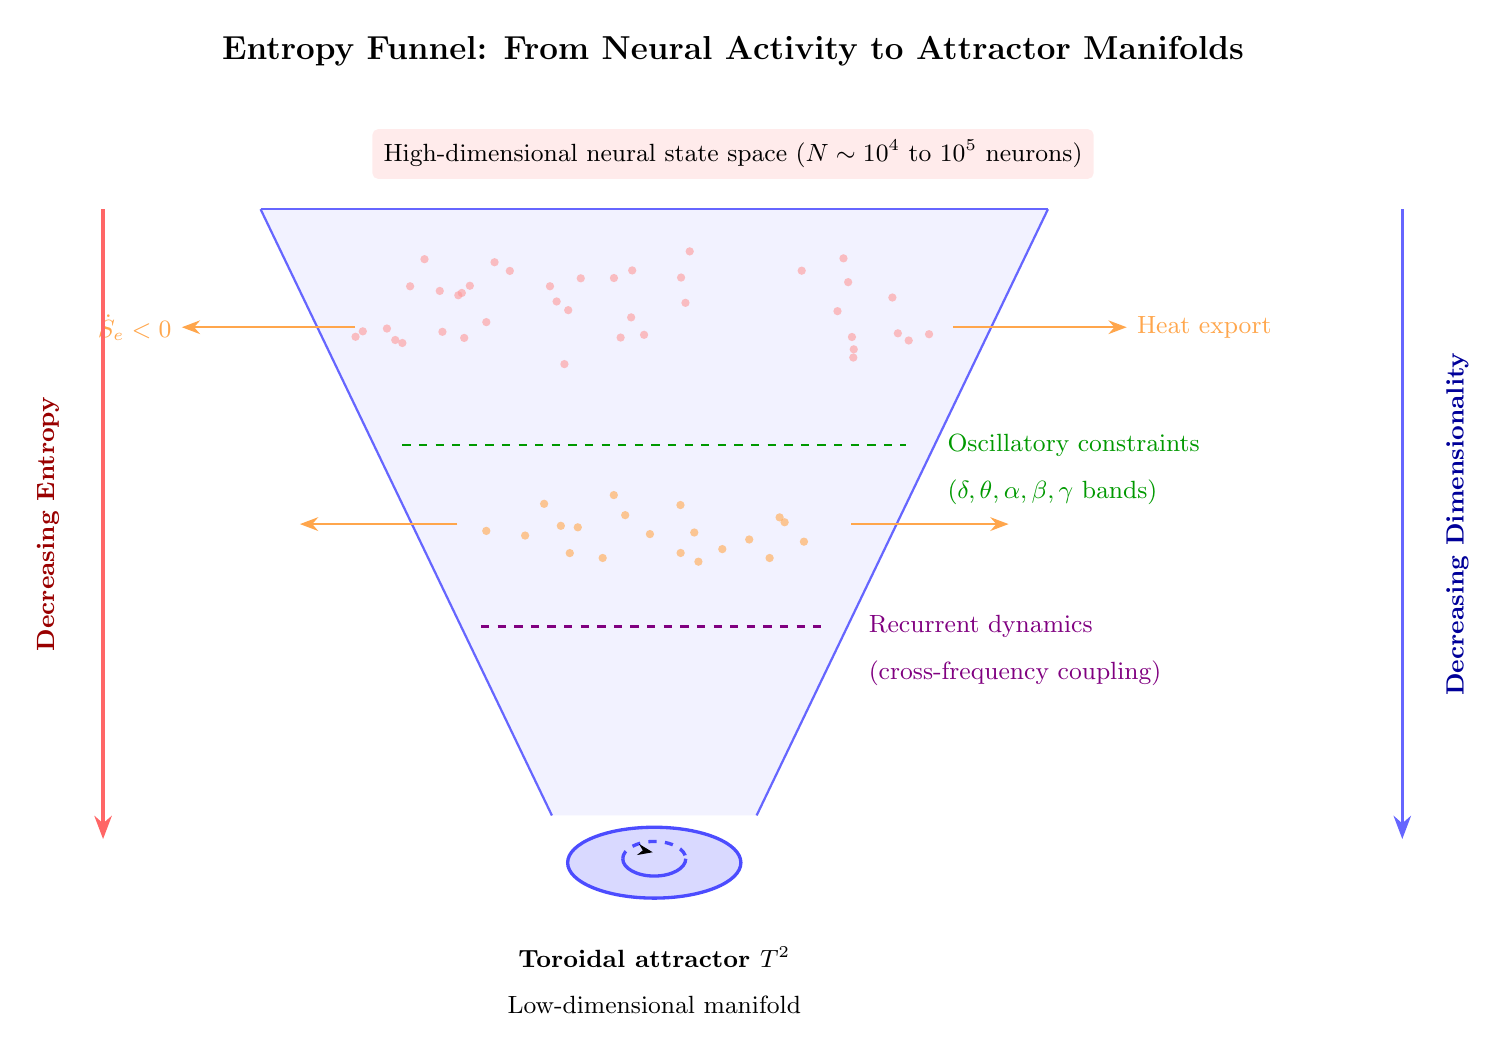
\begin{tikzpicture}[>=Stealth, font=\small]

% Title
\node[font=\large\bfseries] at (1,9.5) {Entropy Funnel: From Neural Activity to Attractor Manifolds};

% ---- Top label ABOVE the funnel ----
\node[font=\small, fill=red!8, rounded corners=2pt, inner sep=4pt] at (1,8.2) 
  {High-dimensional neural state space ($N \sim 10^4$ to $10^5$ neurons)};

% Funnel shape
\fill[blue!5] (-5,7.5) -- (-1.3,-0.2) -- (1.3,-0.2) -- (5,7.5) -- cycle;
\draw[thick, blue!60] (-5,7.5) -- (-1.3,-0.2);
\draw[thick, blue!60] (5,7.5) -- (1.3,-0.2);
\draw[thick, blue!60] (-5,7.5) -- (5,7.5);

% Scattered dots at top (noisy activity) - inside funnel, below top edge
\foreach \i in {1,...,40} {
  \pgfmathsetmacro{\rx}{-3.8 + 7.6*rnd}
  \pgfmathsetmacro{\ry}{5.5 + 1.5*rnd}
  \fill[red!40, opacity=0.6] (\rx,\ry) circle (1.5pt);
}

% Entropy export arrows (well outside funnel)
\draw[->, thick, orange!70] (3.8,6.0) -- (6.0,6.0) node[right, font=\small] {Heat export};
\draw[->, thick, orange!70] (-3.8,6.0) -- (-6.0,6.0) node[left, font=\small] {$\dot{S}_e < 0$};

% Middle layer 1: oscillatory constraints
\draw[thick, dashed, green!60!black] (-3.2,4.5) -- (3.2,4.5);
\node[right, font=\small, green!60!black] at (3.6,4.5) {Oscillatory constraints};
\node[right, font=\small, green!60!black] at (3.6,3.9) {($\delta, \theta, \alpha, \beta, \gamma$ bands)};

% Partially organized dots in middle
\foreach \i in {1,...,20} {
  \pgfmathsetmacro{\rx}{-2.2 + 4.4*rnd}
  \pgfmathsetmacro{\ry}{3.0 + 0.9*rnd}
  \fill[orange!60, opacity=0.7] (\rx,\ry) circle (1.5pt);
}

% Middle export arrows
\draw[->, thick, orange!70] (-2.5,3.5) -- (-4.5,3.5);
\draw[->, thick, orange!70] (2.5,3.5) -- (4.5,3.5);

% Middle layer 2: recurrent dynamics
\draw[thick, dashed, violet] (-2.2,2.2) -- (2.2,2.2);
\node[right, font=\small, violet] at (2.6,2.2) {Recurrent dynamics};
\node[right, font=\small, violet] at (2.6,1.6) {(cross-frequency coupling)};

% Bottom: toroidal attractor
\begin{scope}[shift={(0,-0.8)}]
  \draw[very thick, blue!70, fill=blue!15] (0,0) ellipse (1.1 and 0.45);
  \draw[very thick, blue!70] (-0.4,0.05) arc (180:360:0.4 and 0.22);
  \draw[very thick, blue!70, dashed] (-0.4,0.05) arc (180:0:0.4 and 0.22);
  \draw[thick, red!80, decorate, decoration={markings, mark=at position 0.5 with {\arrow{>}}}] 
    (-0.9,0.1) .. controls (-0.3,0.38) and (0.3,-0.12) .. (0.9,0.15);
\end{scope}

% Toroidal attractor label
\node[font=\small\bfseries] at (0,-2.0) {Toroidal attractor $T^2$};
\node[font=\small] at (0,-2.6) {Low-dimensional manifold};

% Entropy arrow on the left (well outside funnel)
\draw[<-, very thick, red!60] (-7.0,-0.5) -- (-7.0,7.5);
\node[rotate=90, font=\small\bfseries, red!60!black] at (-7.7,3.5) {Decreasing Entropy};

% Dimensionality arrow on the right (well outside all labels)
\draw[<-, very thick, blue!60] (9.5,-0.5) -- (9.5,7.5);
\node[rotate=90, font=\small\bfseries, blue!60!black] at (10.2,3.5) {Decreasing Dimensionality};

\end{tikzpicture}
\end{document}
